\section{Static hand gesture recognition}
\label{sec:handgestures}

The goal of static hand gesture or posture recognition is to recognize hand gestures such as a pointing index finger or the okay-sign based on static data such as images \cite{Oudah20, Yang13}. The current use of hand gesture recognition is primarily in the interaction between computers and humans \cite{Oudah20}. More specifically, typical practical applications can be found in the environment of games, assisted living, and virtual reality \cite{Mujahid21}. In the following, we conduct experiments on a hand gesture recognition dataset constructed by \cite{Mantecon19}, which consists of near-infrared stereo images obtained using the Leap Motion device. First, we crop or segment the images after which we use logistic regression for classification. We see that adversarial logistic regression deteriorates robust generalization with increasing $\epstrain$.

\paragraph{Static hand-gesture dataset}
We use the dataset made available by \cite{Mantecon19}. This dataset consists of near-infrared stereo images taken with the Leap Motion device and provides detailed skeleton data. We base our analysis on the images only. The size of the images is $640 \times 240$ pixels. The dataset consists of $16$ classes of hand poses taken by $25$ different people. We note that the variety between the different people is relatively wide; there are men and women with different posture and hand sizes. However, the different samples taken by the same person are alike.

We consider binary classification between the index-pose and L-pose, and take as a training set $30$ images of the users $16$ to $25$. This results in a training dataset of $300$ samples. We show two examples of the training dataset in Figure \ref{fig:original_examples}, each corresponding to a different class. Observe that the near-infrared images darken the background and successfully highlight the hand-pose. As a test dataset, we take $10$ images of each of the two classes from the users $1$ to $10$ resulting in a test dataset of size $200$.

\begin{figure}
    \centering
    \begin{subfigure}{0.49\textwidth}
    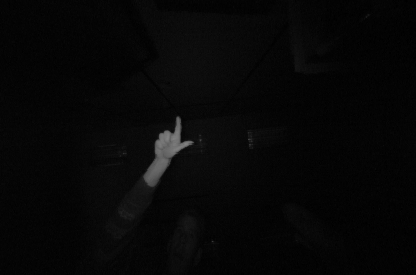
\includegraphics[width=.80\linewidth]{plotsAistats/Lpose.png}
    \caption{L pose}
    \label{fig:L_pose_or_example}
    \end{subfigure}
    \begin{subfigure}{0.49\textwidth}
    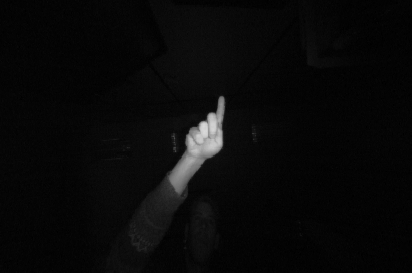
\includegraphics[width=.80\linewidth]{plotsAistats/Indexpose.png}
    \caption{Index pose}
    \label{fig:index_pose_or_example}
    \end{subfigure}
    \caption{We plot two images, where both correspond to the two different classes. We recognize the "L"-sign in Figure \ref{fig:L_pose_or_example} and the index sign in Figure \ref{fig:index_pose_or_example}. Observe that the near-infrared images highlight the hand pose well and blends out much of the non-useful or noisy background. }
\label{fig:original_examples}
\end{figure}

\paragraph{Cropping the dataset}
To speed up training and ease the classification problem, we crop the images from a size of $640 \times 240$ to a size of $200 \times 200$. We crop the images using a basic image segmentation technique to stay as close as possible to real-world applications. The aim is to crop the images such that the hand gesture is centered within the cropped image.

For every user in the training set, we crop an image of the L-pose and the index pose by hand. We call these images the training masks $\{\text{masks}_i \}_{i=1}^{20}$. We note that the more a particular window of an image resembles a mask, the more likely that the window captures the hand gesture correctly. Moreover, the near-infrared images are such that the hands of a person are brighter than the surroundings of the person itself. Based on these two observations, we define the best segment or window, defined by the upper left coordinates $(i,j)$, for an image $x$ as the solution to the following optimization problem:

\begin{equation}
\label{preprocessing}
    \argmin_{i \in [440], \Hquad j \in [40]} \sum_{l=1}^{20}\|\text{masks}_l-x_{\{i:i+200,j:j+200\}}\|^2_2 - \frac{1}{2}\|x_{\{i+w,j+h\}}\|_1.
\end{equation}
Equation \ref{preprocessing} is solved using a full grid search. We use the result to crop both training and test images. Upon manual inspection of the cropped images, close to all images were perfectly cropped. We replace the handful poorly cropped training images with hand-cropped counterparts.

\begin{figure}[!ht]
\centering
\begin{subfigure}{0.31\textwidth}
    \centering
    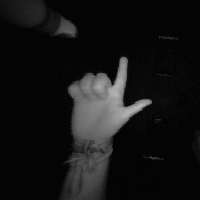
\includegraphics[width=.80\linewidth]{plotsAistats/L_147.png}
    \caption{Cropped L pose}
    \label{fig:cropped_L}
\end{subfigure}
\begin{subfigure}{0.31\textwidth}
    \centering
    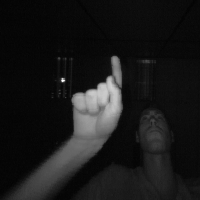
\includegraphics[width=.80\linewidth]{plotsAistats/index_28.png}
    \caption{Cropped index pose}
    \label{fig:cropped_index}
\end{subfigure}
\begin{subfigure}{0.31\textwidth}
    \centering
    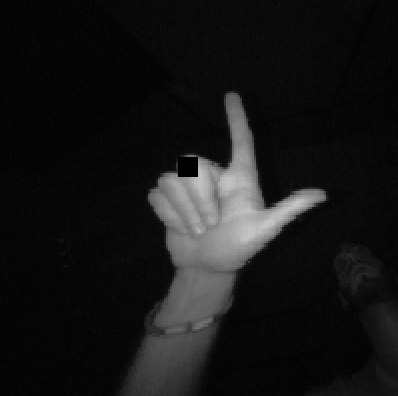
\includegraphics[width=.80\linewidth]{plotsAistats/L_pose_with_mask.png}
    \caption{Black-mask perturbation}
    \label{fig:cropped_L_mask}
\end{subfigure}
    \caption{In Figure \ref{fig:cropped_L} and \ref{fig:cropped_index} we show an example of the images cropped using Equation \ref{preprocessing}. We see that the hands are centered and the images have a size of $200 \times 200$. In Figure \ref{fig:cropped_L_mask} we show an example of the square black-mask perturbation.}
    \label{fig:preprocessing}
\end{figure}

\paragraph{Square-mask perturbations}
 Since we use logistic regression, we perform a full grid search to find the best adversarial perturbation at training and test time. For completeness, the upper left coordinates of the optimal black-mask perturbation of size $\epstrain \times \epstrain$ can be found as the solution to
\begin{equation}
\label{square_perturbations_logistic_regression}
    \text{arg}\max_{i \in [200-\epstrain], \Hquad j \in [200-\epstrain]} \sum_{l,m \in [\epstrain]}\theta_{[i:i+l,j:j+m]}.
\end{equation}
The algorithm is rather slow as we iterate over all possible windows. We show a black-mask perturbation on an $L$-pose image in Figure \ref{fig:cropped_L_mask}.

\paragraph{Results} We run adversarial logistic regression with square-mask perturbations on the cropped dataset and vary the adversarial training budget and plot the result in Figure \ref{fig:eps_mask}. We observe attack that adversarial logistic regression deteriorates robust generalization. 

Because we use adversarial logistic regression, we are able to visualize the classifier. Given the classifier induced by $\theta$, we can visualize how it classifies the images by plotting $\frac{\theta - \min_{i \in [\dims]}\theta_{[i]}}{\max_{i \in [\dims]}\theta_{[i]}} \in [0,1]^{\dims}$. Recall that the class-prediction of our predictor for a data point $(x,y)$ is given by $\text{sign}(\theta^{\top} x) \in \{\pm 1\}$. The lighter parts of the resulting image correspond to the class with label $1$ and the darker patches with the class corresponding to label $-1$.

\begin{wrapfigure}{r}{0.4\textwidth}
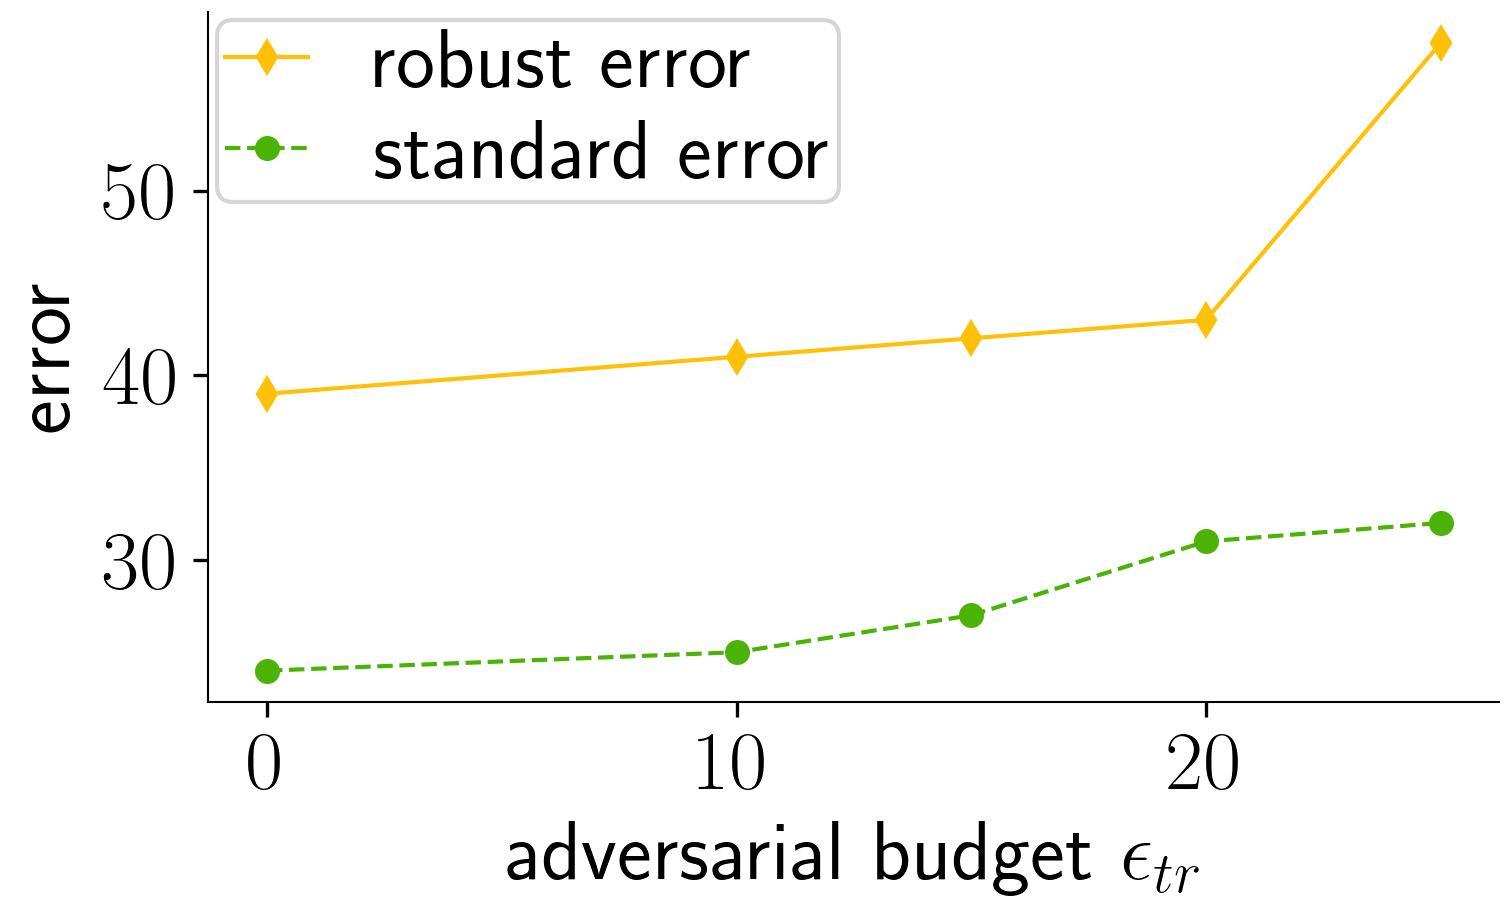
\includegraphics[width=0.99\linewidth]{plotsAistats/mask_plot_main.png}
\caption{We plot the standard error and robust error for varying adversarial training budget $\epstrain$. We see that the larger $\epstrain$ the higher the robust error.}
\label{fig:eps_mask}
\end{wrapfigure}

We plot the classifiers obtained by standard logistic regression and adversarial logistic regression with training adversarial budgets $\epstrain$ of $10$ and $25$ in Figure \ref{fig:visulation_log}. The darker parts in the classifier correspond to patches that are typically bright for the $L$-pose. Complementary, the lighter patches in the classifier correspond to patches that are typically bright for the index pose. We see that in the case of adversarial logistic regression, the background noise is much higher than for standard logistic regression. In other words, adversarial logistic regression puts more weight on non-signal parts in the images to classify the training dataset and hence exhibits worse performance on the test dataset.
 
 \newpage
\begin{figure}[!ht]
\centering
\begin{subfigure}{0.31\textwidth}
    \centering
    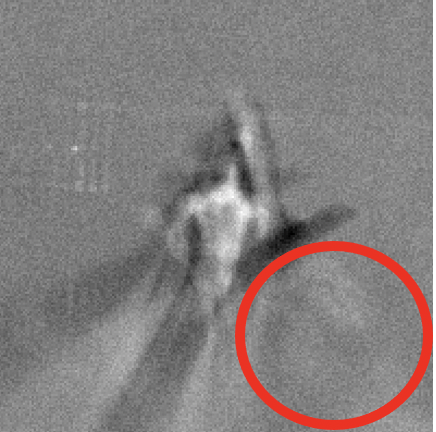
\includegraphics[width=.80\linewidth]{plotsAistats/natural_log_regr_result.png}
    \caption{$\epstrain = 0 $}
    \label{fig:log_natural}
\end{subfigure}
\begin{subfigure}{0.31\textwidth}
    \centering
    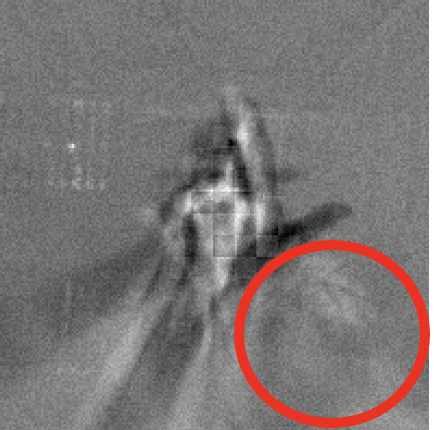
\includegraphics[width=.80\linewidth]{plotsAistats/perTrain10logisticReg.png}
    \caption{$\epstrain = 10 $}
    \label{fig:log_e10}
\end{subfigure}
\begin{subfigure}{0.31\textwidth}
    \centering
    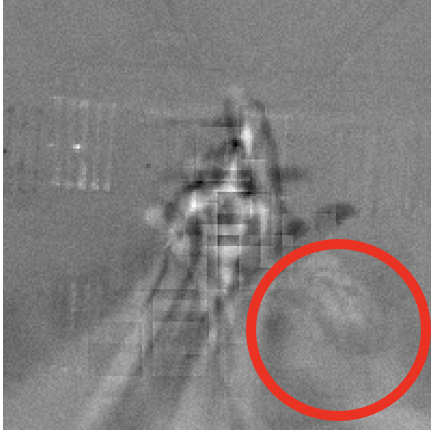
\includegraphics[width=.80\linewidth]{plotsAistats/perTrain25logisticReg.png}
    \caption{$\epstrain = 25$}
    \label{fig:log_e25}
\end{subfigure}
    \caption{We visualize the logistic regression solutions. In Figure \ref{fig:log_natural} we plot the vector that induces the classifier obtained after standard training. In Figure \ref{fig:log_e10} and Figure \ref{fig:log_e25} we plot the vector obtained after training with square-mask perturbations of size $10$ and $25$, respectively. We note the non-signal enhanced background correlations at the parts highlighted with the red circles in the image projection of the adversarially trained classifiers. }
    \label{fig:visulation_log}
\end{figure}
